\documentclass[conference]{IEEEtran}

\usepackage{graphicx}
\usepackage[nolist]{acronym}
\usepackage[backend=bibtex]{biblatex}
\addbibresource{../vision-transformer.bib}

\hyphenation{op-tical net-works semi-conduc-tor}


\begin{document}

\title{ Summery chapter}



\author{\IEEEauthorblockN{Florian Weidner}
	\IEEEauthorblockA{Philipps-University Marburg, Germany\\
		Department of Mathematics and Computer Science, Deep Learning Group\\
		February 09, 2024\\
}}



\maketitle

\begin{abstract}
%\boldmath
The abstract goes here.
\end{abstract}



\IEEEpeerreviewmaketitle



\section{Summary}

\begin{figure}
    \centering
    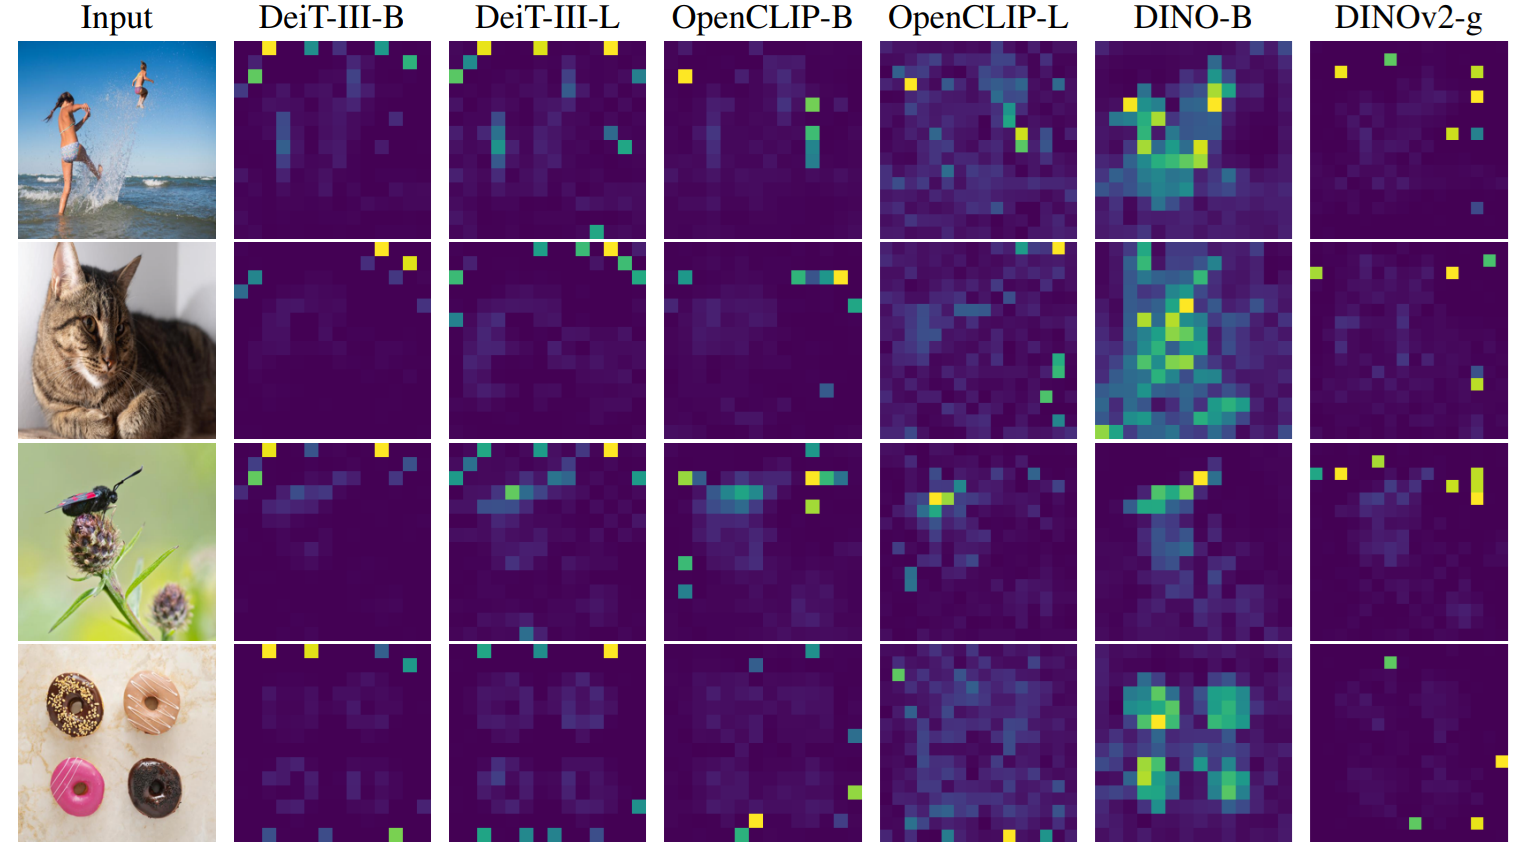
\includegraphics[width=0.5\textwidth]{vits-artifacts.png}
    \caption{Illustration of artifacts observed in the attention maps of modern vision transformers. \cite{registers}}
    \label{fig:artifacts-observations}
\end{figure}

I this chapter we summerize the paper \cite{registers}. The paper discoverd artifacts and proposes to use additional register tokens for \acp{vit} to remove these artifacts.
After introducing to \acp{vit} like we did in this paper, the models they found the artifacts are introduced. The DINO algorithm is a self-supervised learning method, that uses two \acp{vit}. A student network is predicting the output of a teacher network, to learn rich representaions of visual data without the need of manual annotations. \cite{dino} DINO is shown to produce models, that contain semantically consistent information in the last attention layer. Object discovery algorihtms like LOST, built on top of DINO, are using these attention maps, that often contains semantically interpretable information, used to detect objects without supervision. DINOv2 \cite{dinov2} is a improved followup focusing on dense predition tasks, which are tasks, where detailed outputs are required to provide fine-grained localized informations, like semantic segementation or depth estimation. Despite good performance on these dense tasks, the authors observed that DINOv2 is incompatible with LOST \cite{registers}. The different behaviour of DINO and DINOv2 can be observed in the artifacts in the last attention maps. In figure \ref{fig:artifacts-observations} you can see the different models and their artifacts on the last attention layer.
While DINO shows no peak outlier values focusing the main object in the image, DINOv2 shows a lot of artifacts on the background of the images. This qualitatively observation can be also made for the label-supervised model DeiT-III and the text-supervised model OpenCLIP. Shown in figure \ref{fig:artifacts-observations}, you can observe similar artifacts in the background.
To explain why and where the artifacts of \acp{vit} in attention maps appear, the paper focuses on DINOv2. 
Artifact patches show higher norm of their token embedding at the output of the model than other patches. In figure \ref{fig:artifacts-norm} you can see the distribution of the local feature norms over a small dataset. While for DINO, the norm stays under 100 for all patches, DINOv2 shows a lot of patches with a norm higher than 150. This cutoff value can vary across different models. They define artifacts as
\begin{quote}
    "tokens with norm higher than 150 will be considered as “high-norm” tokens" \cite{registers}
\end{quote}

The authors found different conditions, when the artifacts appear in the training process of DINOv2. Figure \ref{fig:artifacts-layer} shows the following conditions:
\begin{itemize}
    \item artifacts start appearing around layer 15 to 40.
    \item artifacts start appearing after on thrid of training.
    \item artifacts only appear in the three largest model versions
\end{itemize}

Another discovery is that the high-norm tokens appear where patch information is redundant. The authors tested the cosine similarity between high-nomr tokens and their four neighbors, directly after the image is emebdded. They observed, that the high norm patches appear where their cosine similarity to the neighbors is high. Compared to the observations, that shows that artifacts appear mostly in the background of images, high-norm pathes seem to have redundant information, that the model can ignore, to achive similar scores at the output. 


\begin{figure}
    \centering
    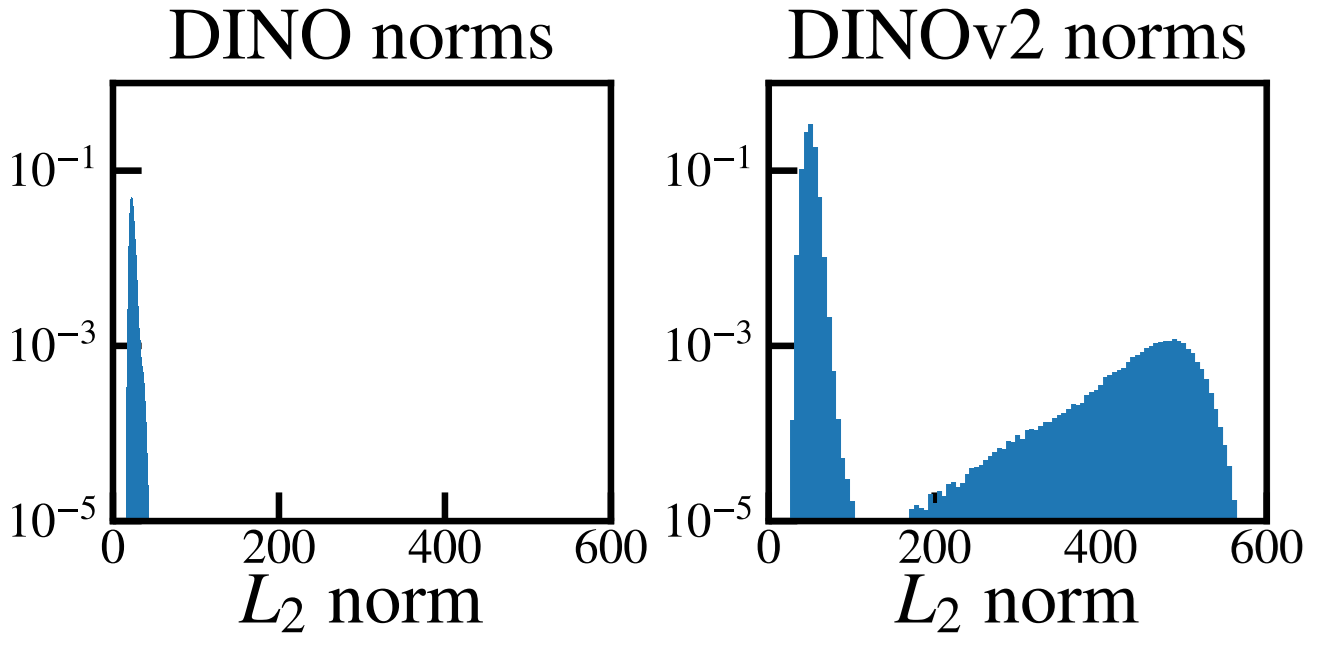
\includegraphics[width=0.3\textwidth]{artifact-norm.png}
    \caption{Comparison of local feature norms for DINO ViT-B/16 and DINOv2 \cite{registers}}
    \label{fig:artifacts-norm}
\end{figure}

\begin{figure}
    \centering
    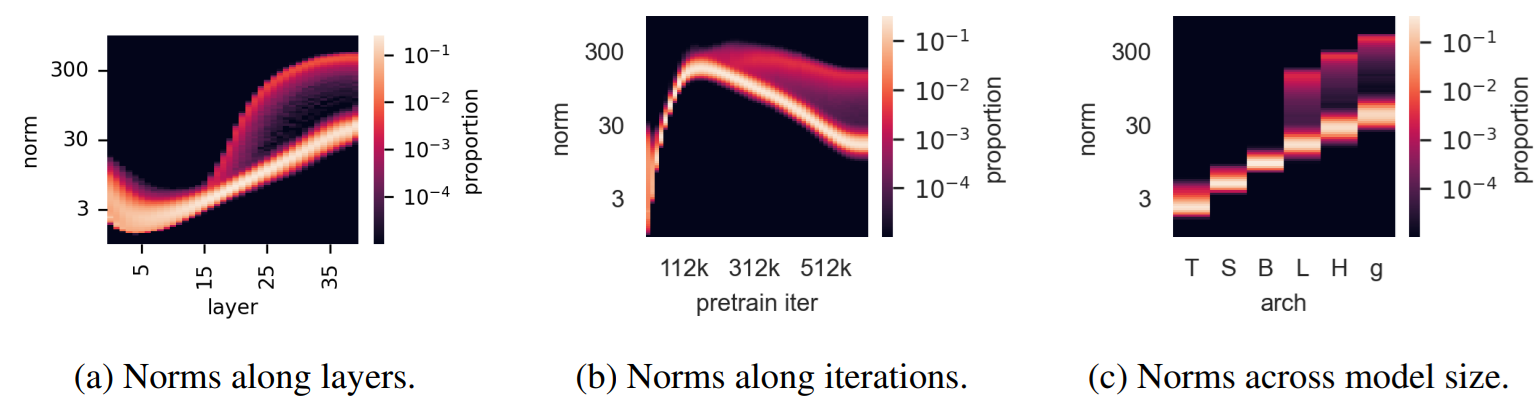
\includegraphics[width=0.5\textwidth]{artifact-layers.png}
    \caption{Illustration of several properties of outlier tokens in the 40-layer DINOv2 ViT-g model \cite{registers}}
    \label{fig:artifacts-layer}
\end{figure}

\printbibliography


\begin{acronym}
	\acro{vit}[ViT]{Vision Transformer}
    \acroplural{vit}[ViTs]{Vision Transformers}
\end{acronym}




% that's all folks
\end{document}


